\chapter{Methods}
\section{The corpus}
Stimuli for the experiments described here were a subset of the \ac{ieee} “Harvard” sentences \citep{HarvardSents} drawn from the \ac{pn/nc} corpus \citep{xxx}.  The sentences in the \ac{pn/nc} corpus were selected based on absence of alliteration or rhyming, avoidance of focus/contrast readings, and lack of marked locutions; The full list of sentences used is given in Appendix~\ref{apx:HarvardSents}.  

Based on within-dialect intelligibility scores from \citet{McCloyEtAl2013}, three talkers were chosen for the present experiments: PNM02, PNM05, and PNM07.  These talkers were selected because, as a group, the Pacific Northwest male talkers exhibited the largest spread in inherent intelligibility in the corpus, and those three talkers formed the endpoints and midpoint of that group (cf. Figure~\ref{fig:dotchart}).

\begin{figure}
	\begin{centering}
	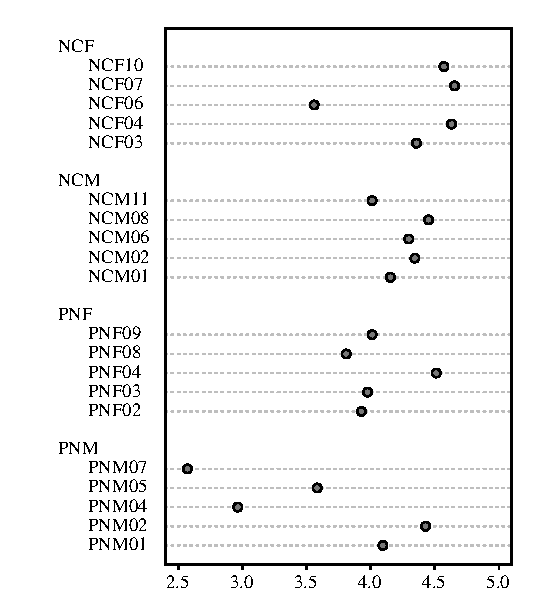
\includegraphics{figures/dotchart.eps}
	\caption[Intelligibility of talkers used to make the stimuli]{By-talker mean keywords correct (across dialect-matched listeners) in speech-shaped noise at +2 dB \ac{snr} (adapted from \citet{McCloyEtAl2013}).\label{fig:dotchart}}
	\end{centering}
\end{figure}

\begin{itm}
	\item{description of the sentences}
	\item{characterization of the talkers}
	\item{results of initial intelligibility study \& acoustic modeling}
	\item{method for selection of the 3 talkers used in the remainder of the experiments}
\end{itm}


\section{Stimulus design\label{sec:StimDesign}}
Why \ac{psola}?  Brief comparison of different methods for manipulating duration.  Malah1979 ("linearly combining adjacent intervals of speech to avoid major discontinuities in the waveform"), MoulinesCharpentier1990 (\ac{psola}).  Relate to the studies that used them: PichenyEtAl1989 (Malah method), UchanskiEtAl1996 (segment-by-segment time scaling), LiuZeng2006 (adding silences, "uniform scaling" = \ac{psola}?).  Cf KrauseBraida2002, KrauseBraida2004.

\begin{itm}
	\item{duration}
	\begin{itm}
		\item{forced alignment}
		\item{hand-correct forced alignment at syllable level}
		\item{auto extract syllable durations from textgrids}
	\end{itm}
	\item{pitch}
	\begin{itm}
		\item{semiauto pitch settings tool}
		\item{auto pitch object extraction}
		\item{auto manipulation from sound \& pitch (save as binary w/ sound)}
		\item{hand-correct pulses within manipulation}
		\item{auto extract point process from manipulation (as text)}
		\item{auto create pitch tier from point process (max interval 0.05s = 20Hz)}
		\item{auto replace pitch tier in manipulation object}
		\item{hand-correct pitch tier (spurious low pitch points)}
	\end{itm}
	\item{intensity}
	\begin{itm}
		\item{auto-extract intensity tier}
		\item{multiply target signal by its conjugate intensity contour}
		\item{dynamic time warp donor intensity contour to match target duration pattern}
		\item{multiply target signal by intensity contour of prosodic source}
	\end{itm}
	\item{PSOLA resynthesis}
	\begin{itm}
		\item{dynamic time warping of intensity tier, pitch tier, and target signal}
		\item{intensity replacement}
		\item{pitch replacement}
	\end{itm}
	\item{final stimulus creation}	
	\begin{itm}
		\item{\ac{rms} normalization}
		\item{create speech shaped noise}
		\item{mix signal and noise — justify chosen \ac{snr}}
		\item{discuss danger of doing \ac{snr} before \ac{rms} — target signal below threshold}
	\end{itm}
\end{itm}


\section{experiment sessions}
Stimuli were presented with a stationary gaussian masker noise, frequency shaped to match the long term spectral average of the corpus of stimuli, at a +2 dB \ac{snr}.  To ensure target audibility, the level of the speech was held constant at 68 dB SPL (dB \ac{rms} in a 6 cc coupler) and the masker noise was digitally added to the speech to achieve the desired \ac{snr}.  The combined signal was presented in a sound-insulated booth over closed-back supra-aural headphones (Sennheiser HD 25–1 II).  Listeners were instructed to repeat each sentence they heard, to give partial answers when they only heard some words, and to guess when they were unsure.  Trials were scored 0–5 on keywords correct during the task.  An audio recording was made of listener responses, and scoring uncertainties were resolved offline by a second researcher.  Talker-sentence-\ac{snr} assignments were random and unique for each listener, with the following constraints: (a) each listener heard each talker an equal number of times; (b) within each talker, each listener heard each \ac{snr} an equal number of times; (c) each listener heard each sentence only once.

\begin{itm}
	\item{subjects}
	\begin{itm}
		\item{number of listeners}
		\item{hearing test}
		\item{dialect controls}
		\item{demographics: age, gender, ethnicity, geography}
		\item{English native; other languages?}
	\end{itm}
	\item{procedure}
	\begin{itm}
		\item{booth, headphones, presentation level}
		\item{task}
		\item{scoring}
	\end{itm}
\end{itm}

\section{data analysis}
\begin{itm}
	\item{mixed effects models (probably logistic)}
\end{itm}
